\chapter{Resultados}
\section{Pruebas de estimación de posición y velocidad}
	Dicho en el capítulo anterior, el nodo de cálculo de la posición del balón se encarga de obtener las posiciones $X$ y $Y$, por lo que un script de Python llamado $graph_-kalman_-estimator.py$ grafica las pocisiones exactas, calculadas, predichas y corregidas por el EKF para hacer una comparación mejor observable de los datos y fiabilidad del filtro. Véase la Figura \ref{fig:estimator_graphics}.
	
\begin{figure}
\centering
	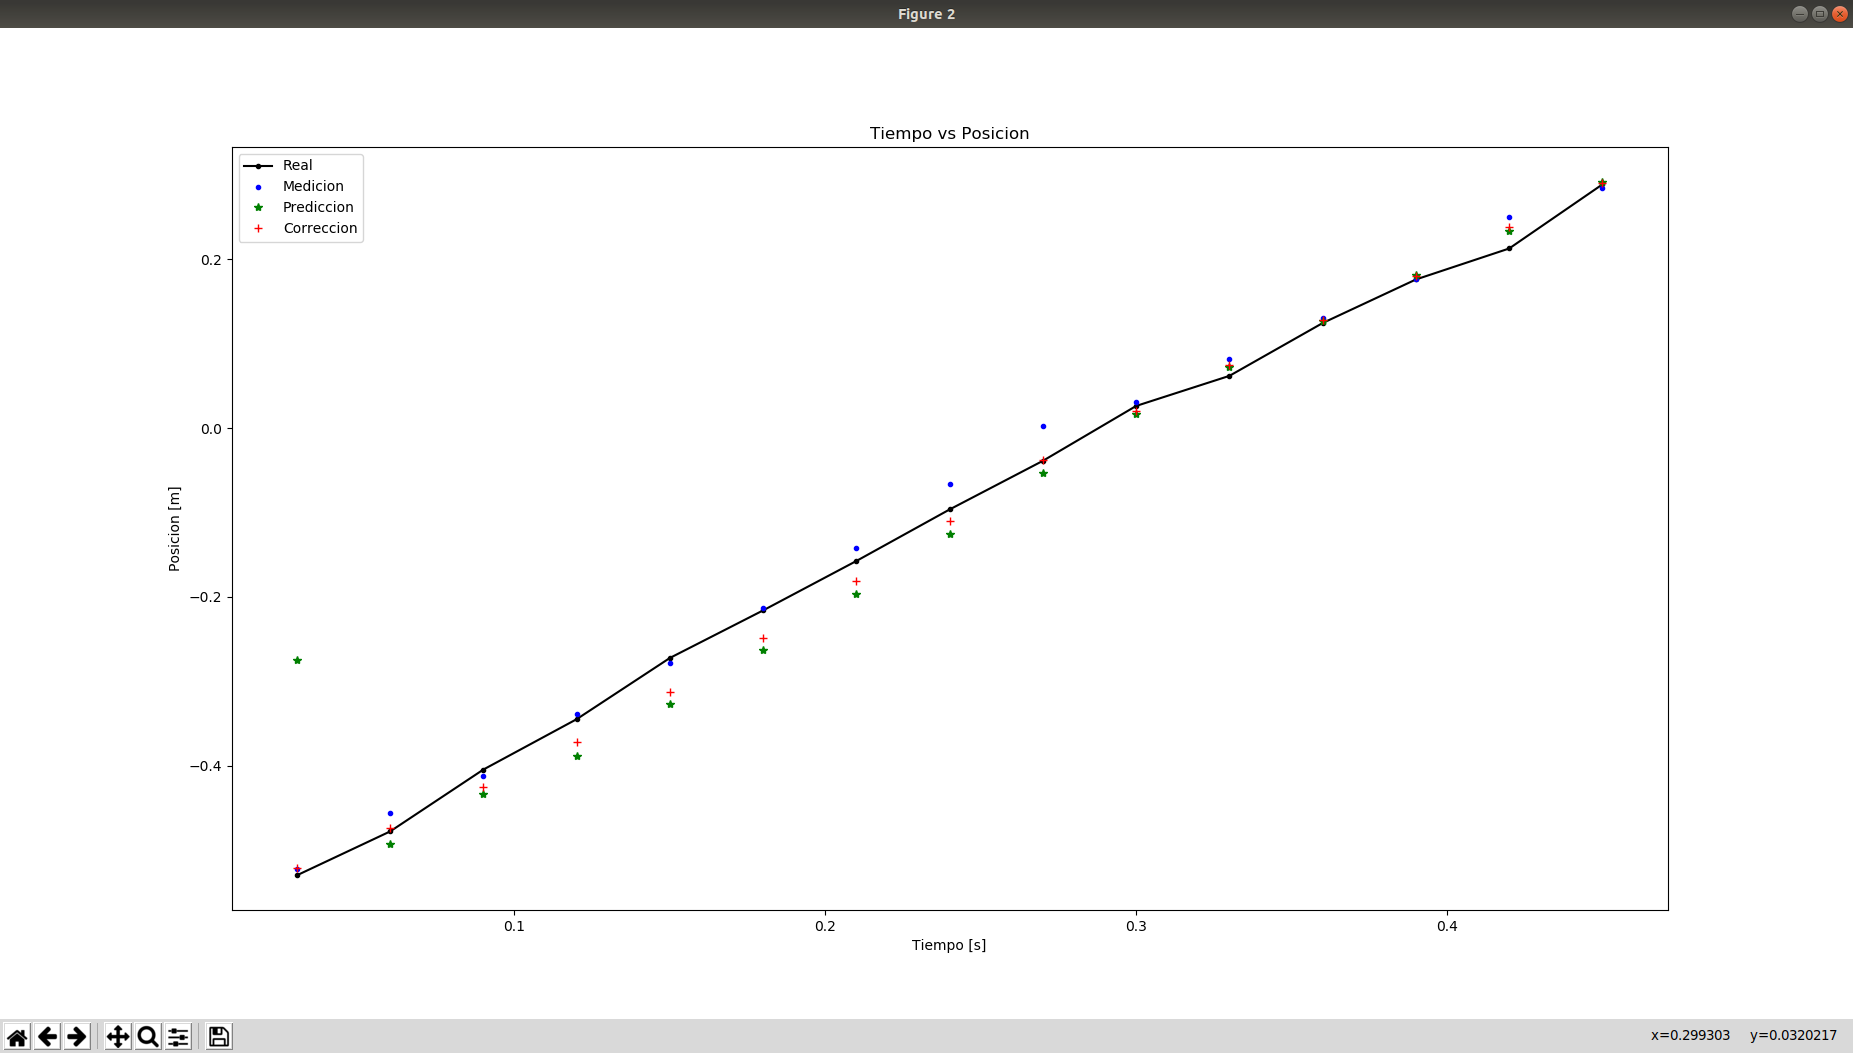
\includegraphics[scale=0.15]{images/data_1.png}
	\caption{Gráfica de comparación de la pocición real, medida, predicha y corregida a lo largo de un muestreo de tiempo a 30 Hz.}
\label{fig:estimator_graphics}
\end{figure}

\section{Pateo de un balón como prueba del sistema completo}

	La finalidad de este trabajo de tesis no es limitarse al análisis teórico, dado que el robot está diseñado para competencias internacionales, por lo que una forma sencilla y útil de implementarla es haciendo la prueba del \textit{RoboCup} llamada \textit{kick from a moving ball}. Esta prueba puede verse en la Figura: \ref{fig:final_test}.
	
\begin{figure}
\centering
	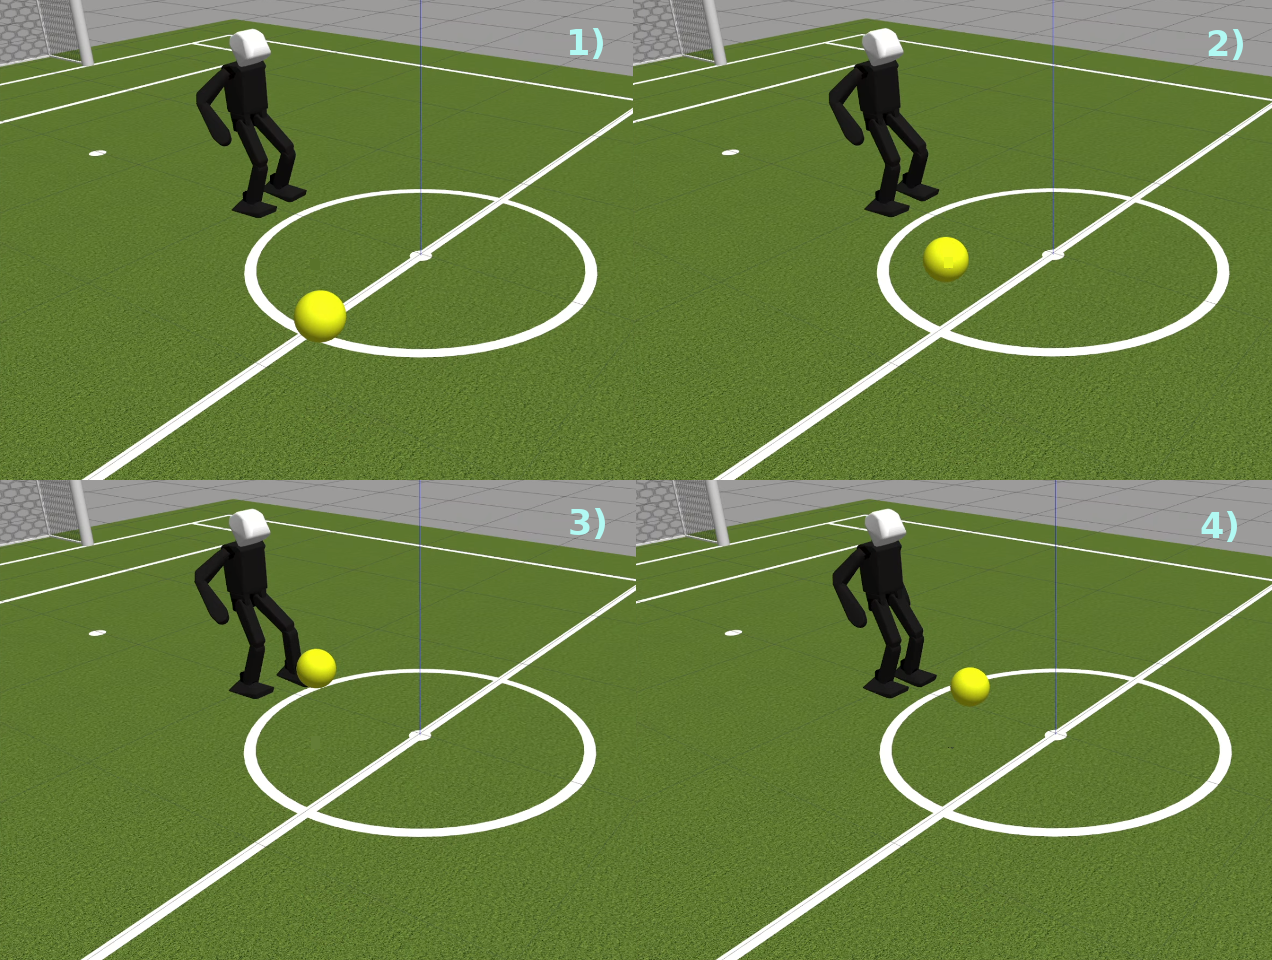
\includegraphics[scale=0.2]{images/final_test.png}
	\caption{Secuencia que ilustra el pateo del balón en movimiento como implementación del filtro.}
\label{fig:final_test}
\end{figure} 